\chapter{Radio Astronomy and the Rotation of the Galaxy (Small Radio Telescope)}

%todo
% - Add information on how students can infer existance of dark matter from rotation curve
% - rewrite lab manual so it presents goals of project
% - for negative longitude, should be blueshifted, not redshifted.
% - for evening labs or others where -90<l<90 is not in range, then can examine spectra on either sides of l=180, they should be reflections of each other (one red shifted, one blue shifted)
% - for the last question, resolution should be 4 degrees, not 9.

\section{Assessment}

Your lab report will be assessed based on answering lab questions correctly and with justification (showing work or giving reasoning) and the following rubric rows found in Appendix~\ref{cha:rubrics}: A11, F2, G4, G5.

\section{Changes to the lab write-up}

The lab write-up is included below, and the following changes should be made to it.

\subsection{Operating the small radio telescope (page 3)}

The telescope is mounted 3\textdegree{} azimuth out of alignment. Each time the SRT program is loaded, the following command must be run to compensate for this, before any useful observations can be made.

\begin{itemize}
	\item Click on the ``\texttt{offset}'' button in the top row.
	
	\item Type ``\texttt{3.0 0.0}'' and press enter.
\end{itemize}

\section{Lab write-up}

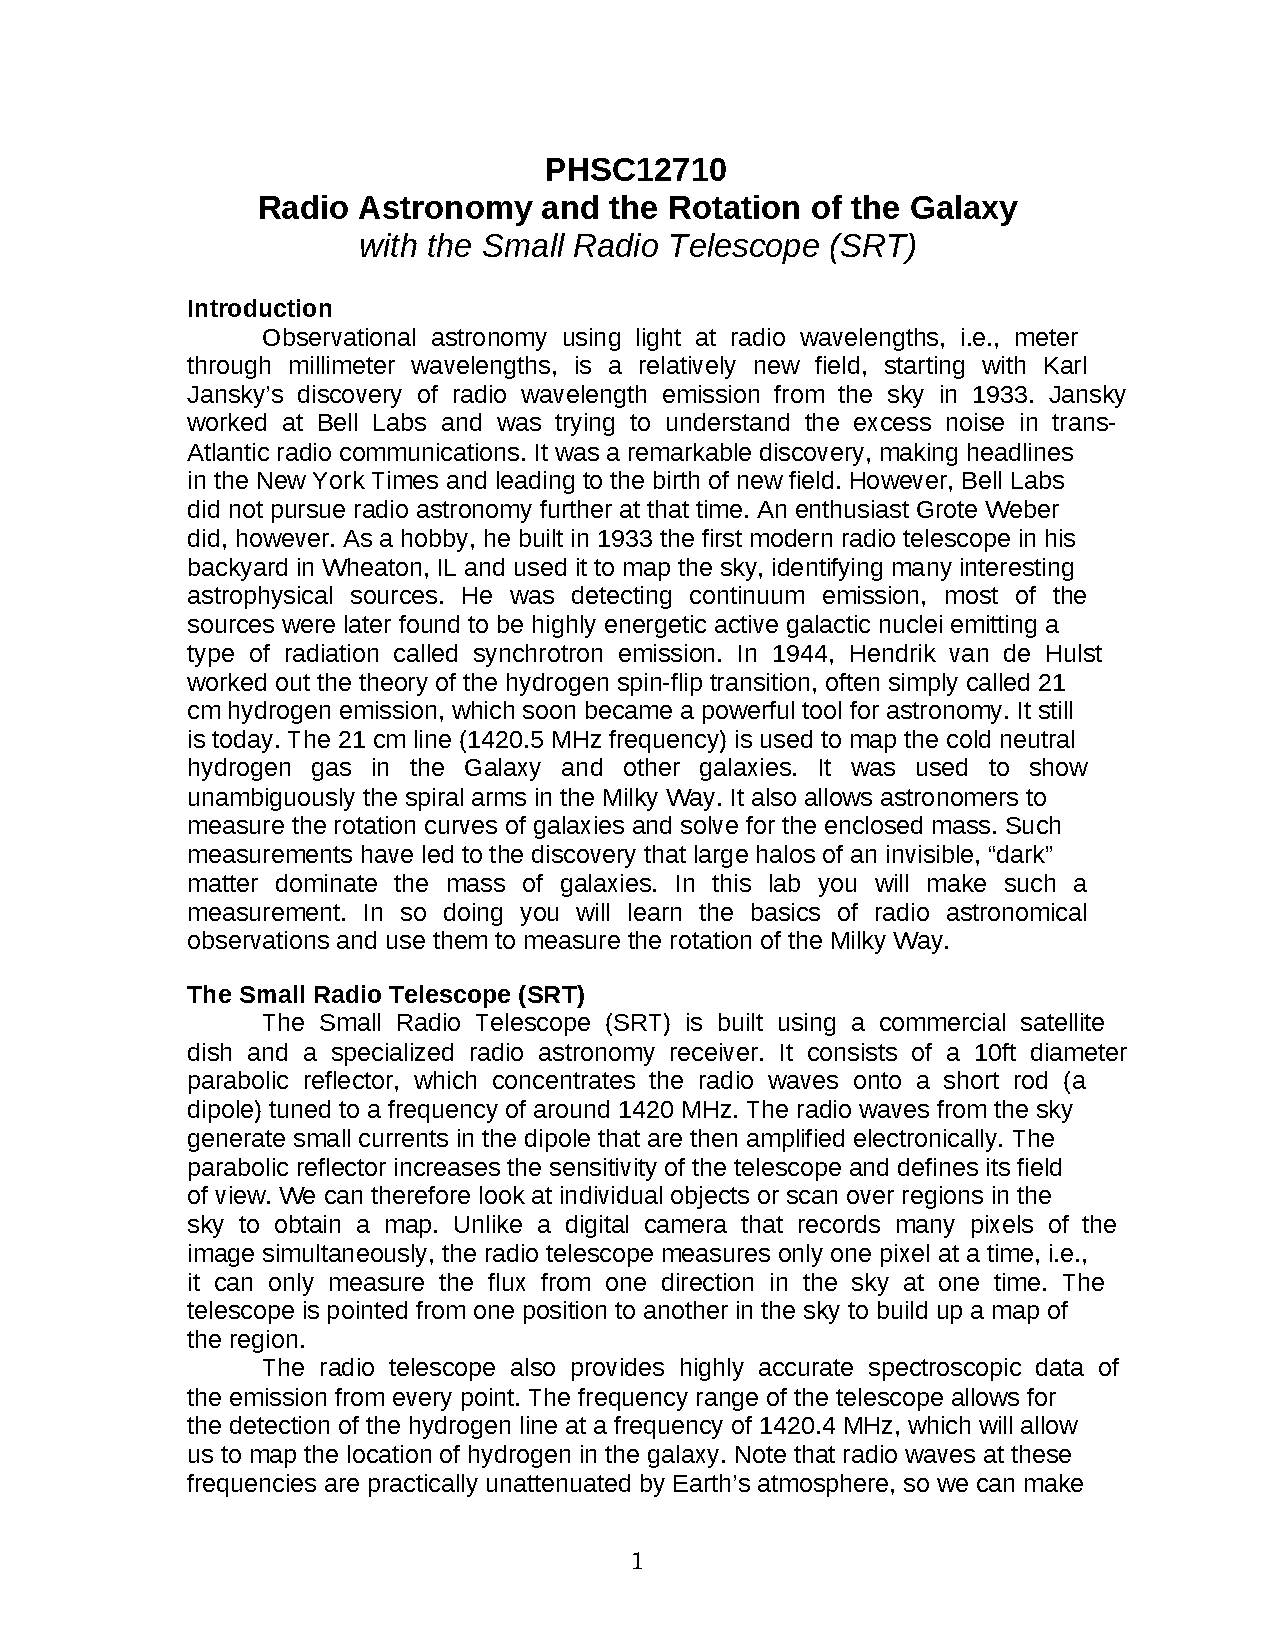
\includepdf[pages=-]{galaxy-rotation-srt/MilkyWayLab.pdf}